
\chapter{Materiais e Métodos}

\section{Datasets}

Bases de dados para treinamento ou teste de algoritmos de estimação de profundidade consistem em imagens RGB de uma cena e sua anotação correspondente em profundidade. Ao longo do tempo, diversos \textit{datasets} foram propostos para este fim com variações em formatos de anotações, tipos de cena (interior ou exterior), métodos de captura, qualidade, resolução e tamanho.

% \textcolor{red}{colocar citações que tem na seção 3 do midas 1}.

Geralmente são empregados sensores e outras tecnologias como \textit{Stereo Matching} e \textit{Structure from Motion} para criar os \textit{datasets} de profundidade, porém, são abordagens muito complexas, custosas, ou inviáveis em algumas situações particulares, por exemplo, obter mapas de profundidades densos a partir de veículos em movimento  \cite{yang2024depthv1}.
Cada \textit{dataset} possui suas próprias características, problemas e vieses. Dados com informação de profundidade e em alta qualidade são complexos de adquirir, sendo que os melhores conjuntos são utilizados no treinamento dos modelos presentes na literatura \cite{ranftl2020towards}. 



Dessa forma, para escolha das bases de dados a serem utilizadas para teste, temos os critérios: i) não ter composto o conjunto de treinamento dos modelos escolhidos para comparação, ii) conter dados válidos para avaliação considerando anotações precisas de profundidade, ou caso sejam esparsas, possuam máscara para indicar os pixels válidos, iii) ser uma base de dados conceituada na literatura. Os \textit{datasets} escolhidos e suas características podem ser visualizados na Tabela \ref{tabdata}.

% PESQUISA ANTIGA -------------------------------------------------------------------
% O presente trabalho exige um tipo de base de dados pouco encontrado na literatura, trios de imagem RGB, mapa de profundidade com erros e um outro mapa de profundidade denso e completo. De acordo com \cite{zhang2018deep}, uma das maneiras de se obter esses dados seria capturar imagens com uma câmera RGB-D de baixo custo e alinha-las com outra captura simultânea de um sensor mais preciso, porém essa abordagem é muito custosa, além de que não há disponibilidade de grandes conjuntos para treinamento.

% O presente projeto pretende utilizar como base de dados principal o \textbf{Hypersim}. Um \textit{dataset} para compreensão de cenas baseado em cenas sintéticas fotorrealistas. Contendo 77.400 imagens de 461 cenas \textit{indoor} com pares de RGB e mapas de profundidade calculado deterministicamente, além de outras informações como normais de superfície, rótulos de segmentação e detecção de objetos e entre outros \cite{roberts2021hypersim}.
% PESQUISA ANTIGA -------------------------------------------------------------------


% Please add the following required packages to your document preamble:
% \usepackage{graphicx}
\begin{table}[h]
    \centering
    \caption{Características dos datasets utilizados no trabalho}
    \label{tabdata}
    \resizebox{\textwidth}{!}{%
    \begin{tabular}{ccccccc}
    \hline
    \textbf{Dataset} & \textbf{Sensor} & \textbf{Anotação} & \textbf{Tipo} & \textbf{Cenário} & \textbf{Num. Imagens} & \textbf{Resolução} \\ \hline
    KITTI  & LiDAR         & Esparsa & Real      & Outdoor        & 44 K   & 1024 $\times$ 320  \\
    Nyu-V2 & Kinect V1     & Densa   & Real      & Indoor         & 1449   & 640 $\times$ 480   \\
    DIODE  & Laser Scanner & Densa   & Real      & Indoor/Outdoor & 25,5 K & 768 $\times$ 1024  \\
    SINTEL & -             & Densa   & Sintético & Indoor/Outdoor & 1064   & 1024 $\times$ 436  \\
    ETH3D  & Laser Scanner & Densa   & Real      & Indoor/Outdoor & 454    & 6048 $\times$ 4032 \\ \hline
    \end{tabular}%
    }
    \end{table}


\subsection{NYUv2}


%% refazer o texto

O \textit{dataset} NYUv2 é um dos mais utilizados em tarefas de visão computacional que envolvam estimação de profundidade, segmentação de cenas e reconhecimento de objetos. Possui 1449 pares de imagens RGB e mapas de profundidade densos em diversas cenas \textit{indoor} divididos em 795 para treinamento e 654 para teste \cite{silberman2012indoor}. A resolução das imagens é de 640 $\times$ 480 pixels. O equipamento de aquisição foi o Microsoft Kinect que utiliza a técnica de ToF ponto a ponto, que produz resultados precisos de informação de profundidade. Além dos pares RGB-D, também são disponibilizados os dados brutos de leitura dos sensores em que é possível encontrar aproximadamente 70\% de pixels com informação válida de profundidade, no entanto, as imagens finais foram processadas utilizando um método de correção, resultando em um mapa denso,  Além das informações de profundidade, a base de dados provém rótulos de segmentação de objetos e relações de suporte \cite{lahiri2024deep}, como observado na Figura \ref{exnyuv2} que ilustra um exemplo. Entre as cenas observadas, podemos citar cômodos comuns de casas como quartos, cozinhas, sala de aula, banheiro e etc \cite{silberman2012indoor}.

\begin{figure}[h!]
    \centering
    \caption{Exemplo do \textit{dataset} NYU Depth v2}
    \includegraphics[width=.8\textwidth]{fig/example_nyu.png}
    \caption*{Fonte: \textit{Dataset} NYU Depth V2, do trabalho de \citeonline{silberman2012indoor}}
    \label{exnyuv2}
\end{figure}

\newpage

\subsection{KITTI}

Com o objetivo de impulsionar o desenvolvimento da área de veículos autônomos, o trabalho de \citeonline{Geiger2012CVPR} apresenta o \textit{benchmark} KITTI. Este \textit{benchmark} possui bases de dados para diversos tipos de tarefas de visão computacional relacionadas à navegação de veículos, tais como, visão estéreo, fluxo ótico, correção de mapas de profundidade, estimação de profundidade, odometria, detecção de objetos 2D e 3D, rastreamento de veículos e pessoas, detecção de pavimentação urbana e segmentação semântica. 



Os dados foram capturado por meio de um veículo equipado com diversos tipos de sensores, por exemplo, câmeras RGB, scanner a laser, GPS (\textit{Global Positioning System}) de alta precisão e IMU (\textit{Inertia Measurement Unit}). Além disso, as imagens RGB utilizando um par de câmeras em estereoscopia e os dados de profundidade foram adquiridos com um sensor Velodyne HDL-643 que utiliza tecnologia LiDAR. Os rótulos providos por esse sensor são esparsos, apresentando aproximadamente 30\% de pixels válidos em cada imagem. A resolução das imagens da base de dados de estimação de profundidade possuem resolução de 1216 $\times$ 352 \cite{lahiri2024deep}. Um dos exemplos do \textit{dataset} pode ser visualizado na Figura \ref{fig:kittiexample}, em que podemos observar um mapa de profundidade esparso e a imagem RGB correspondente.

\begin{figure}[h]
    \centering
    \caption{Exemplo do \textit{dataset} KITTI de estimação de profundidade}
    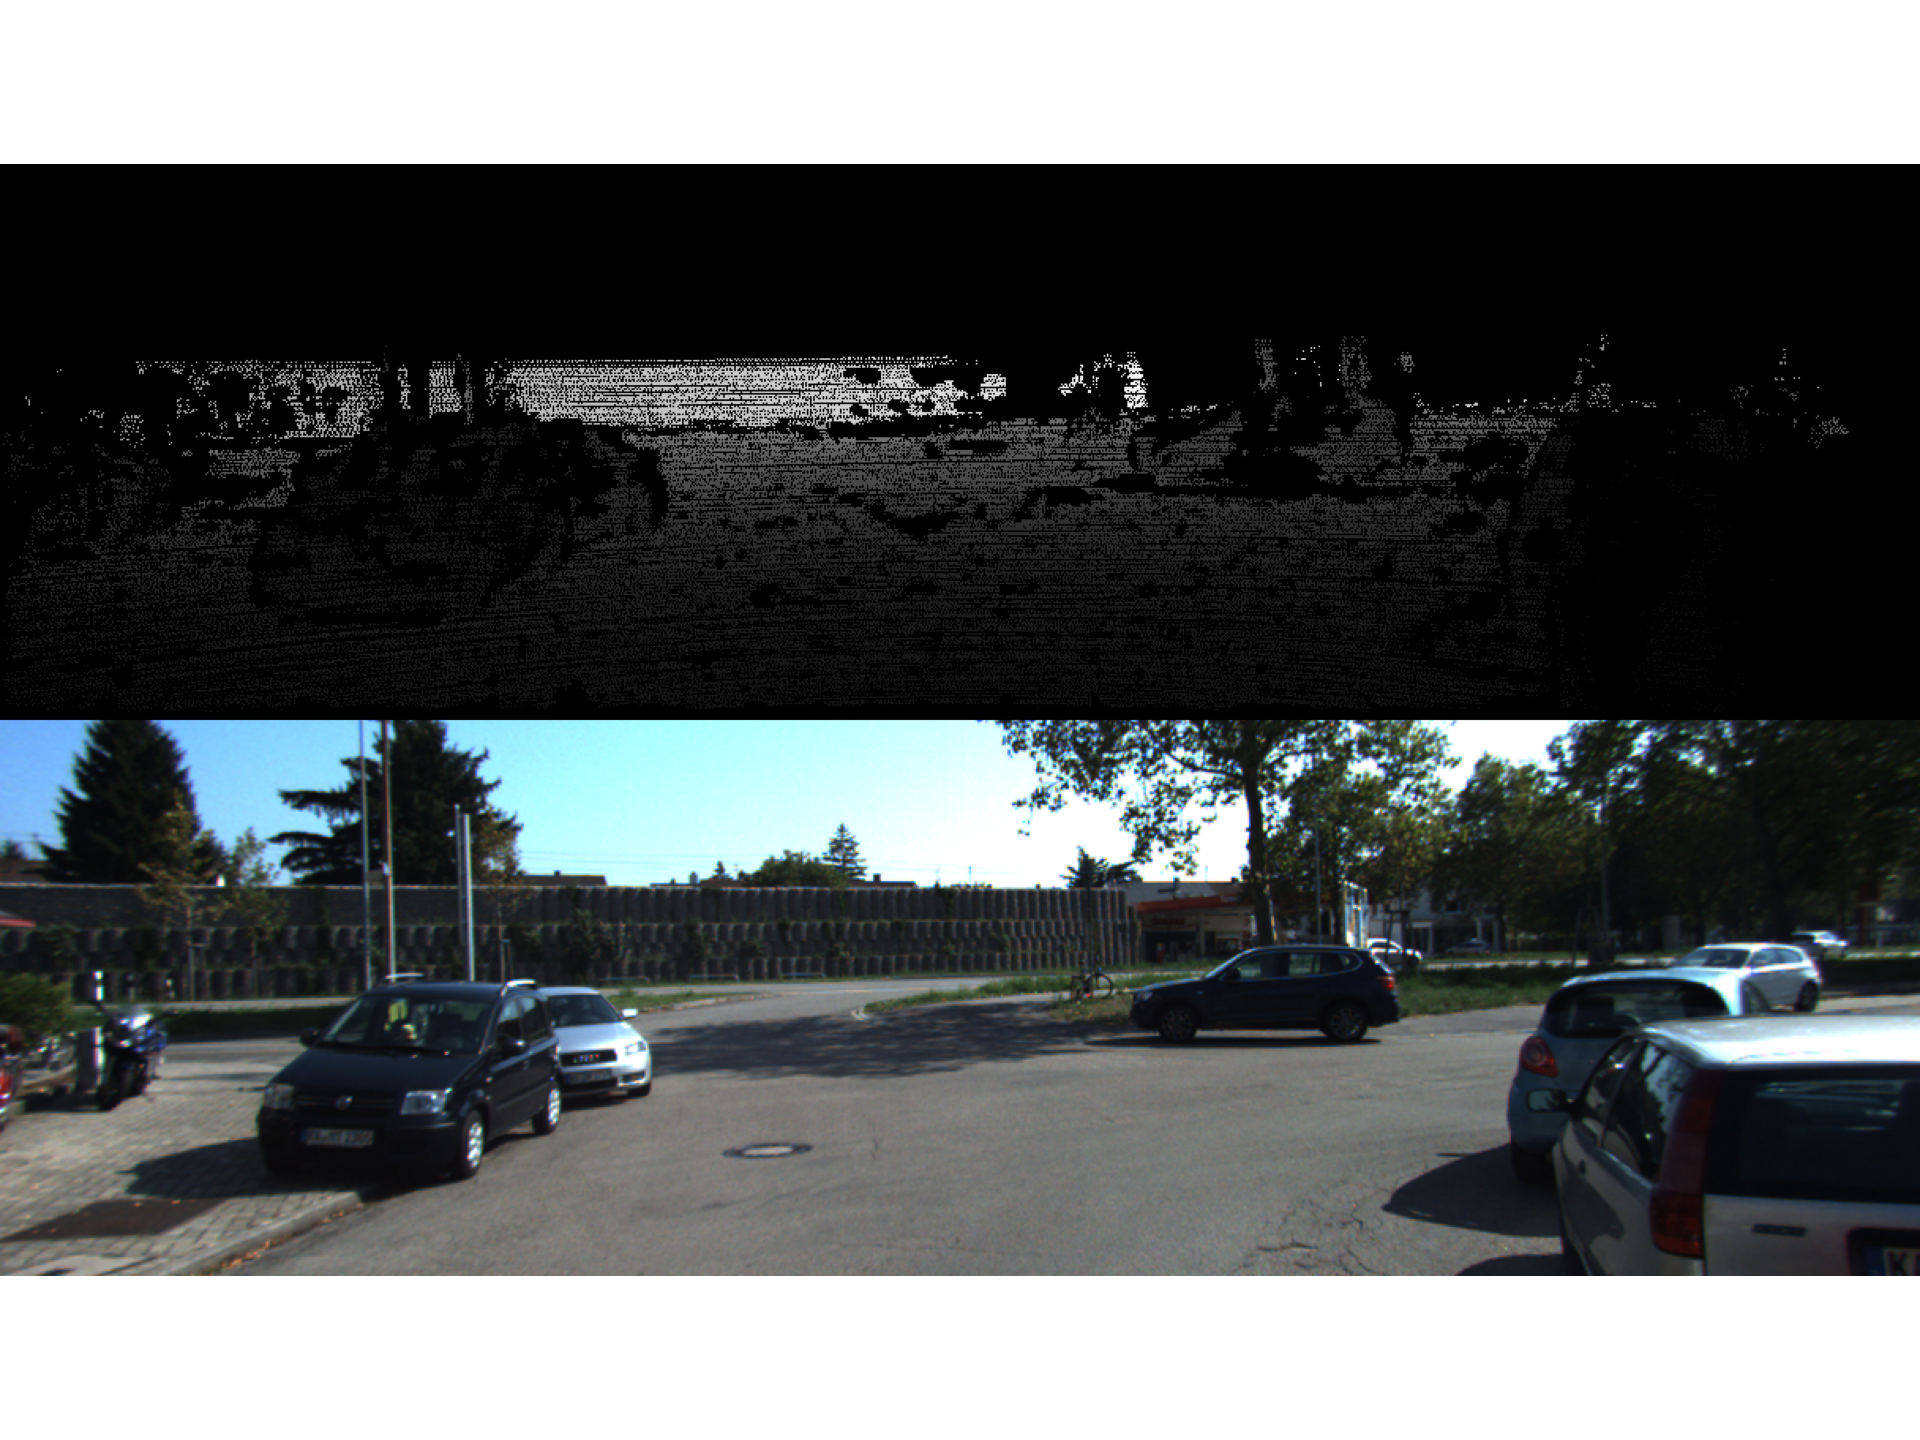
\includegraphics[width=.8\textwidth]{fig/example_kitti.png}
    \caption*{Fonte: \textit{Dataset} KITTI, do trabalho de \citeonline{Geiger2012CVPR}}
    \label{fig:kittiexample}
\end{figure}

\newpage

\subsection{SINTEL}

O Sintel é uma base de dados sintéticos criada a partir de uma projeto aberto de animação em CGI (\textit{Computer-Generated Imagery}) chamado \textit{Durian Open Source Movie Project}. Foi elaborado no \textit{software} Blender e contém os arquivos fontes utilizados na criação do filme animado. Em \cite{Butler:ECCV:2012}, os autores adaptaram os arquivos brutos em uma base de dados primariamente utilizada para o problema de visão computacional de estimação de fluxo ótico. Apesar do seu uso primário ser em outra tarefa, ele também contém anotações de profundidade das imagens. A Figura \ref{fig:sintelexample} mostra um quadro renderizado e seu mapa de profundidade calculado.

\begin{figure}[h]
    \centering
    \caption{Exemplo do \textit{dataset} Sintel}
    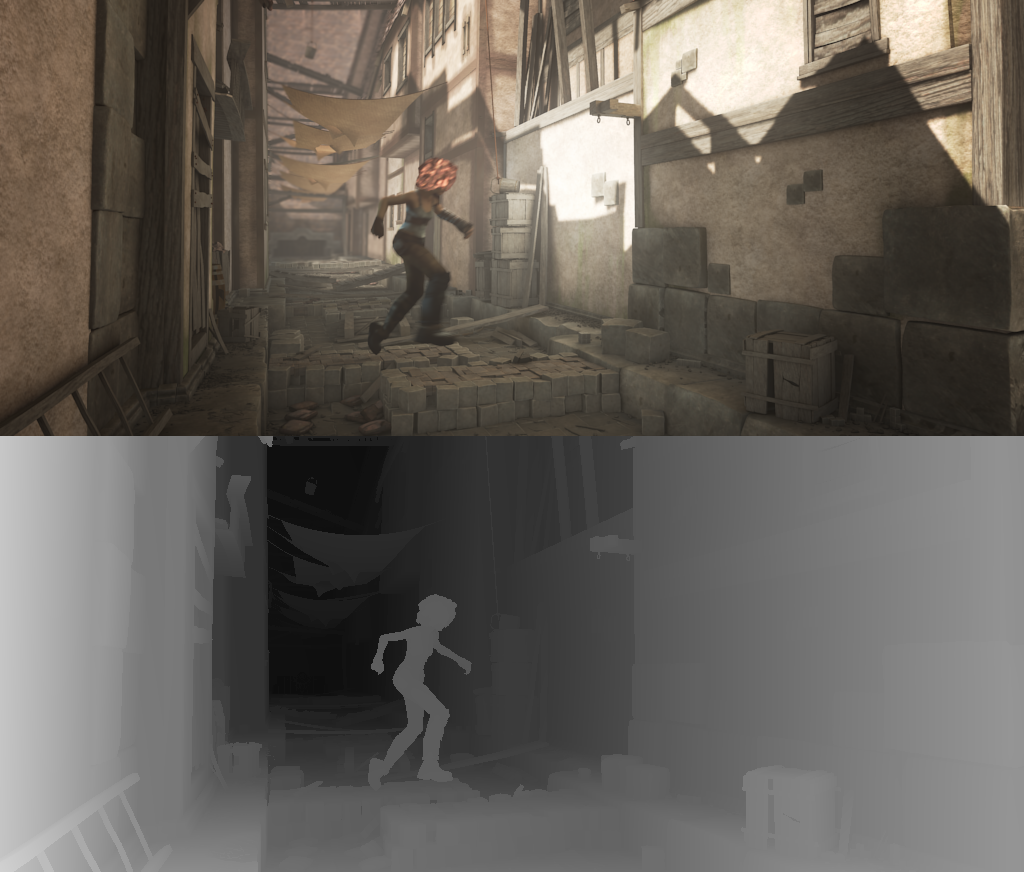
\includegraphics[width=.6\textwidth]{fig/sintel_example.png}
    \caption*{Fonte: \textit{Dataset} Sintel, do trabalho de \citeonline{Butler:ECCV:2012}}
    \label{fig:sintelexample}
\end{figure}


A base de dados contém um total de 35 cenas, cada uma possuindo entre 20 a 50 quadros, totalizando 1628 imagens. A resolução de renderização é de 1024 $\times$ 436 em 24 FPS (\textit{Frames Per Second}). As cenas possuem como características presentes efeitos atmosféricos, efeitos de movimento, desfoque em razão de velocidade e alta variabilidade de ambientes, personagens e ações. É dividido em 1064 quadros para o conjunto de treinamento e 564 para teste, sendo anotadas apenas as imagens de treinamento \cite{wulff2012lessons}. 



\subsection{ETH3D}

O ETH3D é uma base de dados geralmente utilizada para reconstrução em vistas múltiplas e \textit{stereo matching}. Contém dados de treinamento com imagens RGB \textit{multiview}, capturadas com câmeras DSLR (\textit{Digital Single Lens Reflex}) e anotações de profundidade capturadas utilizando um scanner a laser Faro Focus X 330. Oferece três versões de imagens de profundidade, uma correspondente à leitura bruta do sensor (\textit{raw}), outra com valores extremos removidos por trabalho manual e uma ferramenta automática (\textit{clean}) e uma com valores extremos e pontos observados por uma única imagem RGB removidos. A partição de teste não contém anotações. A base de dados é associada à um desafio aberto ao público. Inclui cenas tanto internas quanto externas, oferecendo um protocolo de avaliação bem variado \cite{lahiri2024deep} \cite{schops2019bad}. 

\begin{figure}[h]
    \centering
    \caption{Exemplo do \textit{dataset} ETH3D}
    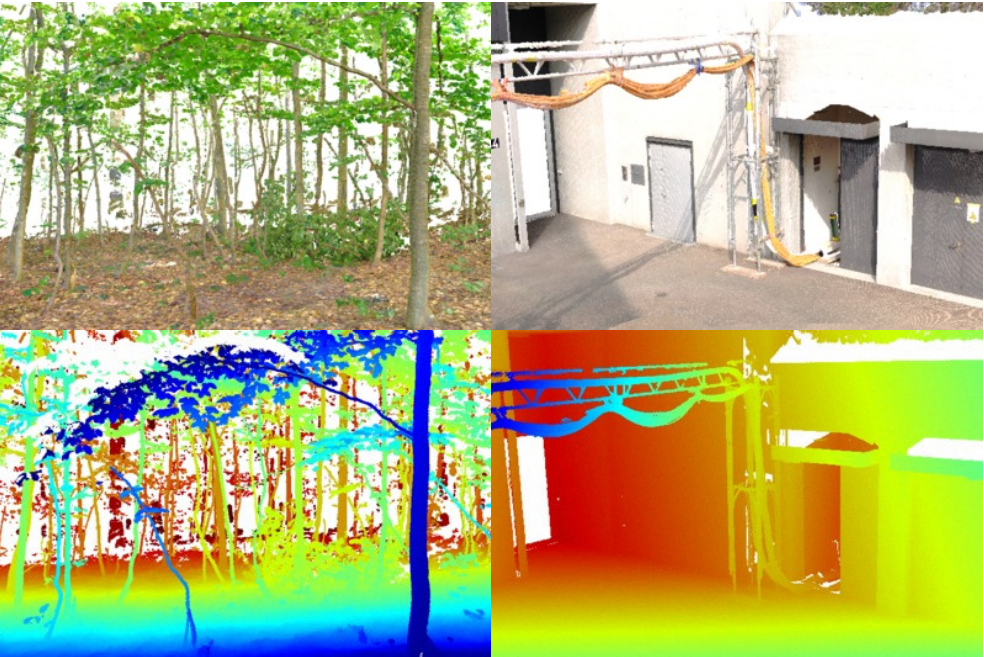
\includegraphics[width=.6\textwidth]{fig/eth3d_example.png}
    \caption*{Fonte: \textit{Dataset} ETH3D, do trabalho de \citeonline{schoeps2017cvpr}}
    \label{fig:eth3dexample}
\end{figure}


\subsection{DIODE}

O \textit{dataset} DIODE (\textit{Dense Indoor and Outdoor Depth Dataset}), é uma base de dados para estimação monocular de profundidade e possui cerca de 8.000 imagens de ambientes internos e 16.000 de ambientes externos para treinamento e teste. Possui resolução de 768 $\times$ 1024 com faixa de distâncias entre 50m e 300m para os ambientes internos e externos respectivamente. O equipamento de aquisição é o scanner a laser Faro Focus S350. Alguns exemplos do \textit{dataset} podem ser visualizados na Figura \ref{exdiode} \cite{diode_dataset}.

\begin{figure}[h]
    \centering
    \caption{Exemplo do \textit{dataset} DIODE}
    \includegraphics[width=\textwidth]{fig/example_diode.png}
    \caption*{Fonte: \textit{Dataset} DIODE, do trabalho de \citeonline{diode_dataset}}
    \label{exdiode}
\end{figure}



\section{Protocolo de Avaliação}

Para avaliar os modelos de estimação de profundidade, será utilizado o protocolo de \textit{zero-shot cross-dataset transfer}, i.e. realizar os testes e métricas em bases de dados que não compuseram os conjuntos de treinamentos dos modelos analisados. A performance em \textit{cross-dataset} é considerada uma aproximação mais fiel da performance em mundo real em uma aplicação, pois os conjuntos de testes relativos aos conjuntos utilizados no treinamento podem refletir os mesmos vieses e situações \cite{ranftl2020towards}.

Há dois tipos de métricas usadas para avaliação de mapas de profundidade, a acurácia de profundidade e o erro métrico de profundidade. Apesar do problema de MDE ser caracterizado como uma tarefa de regressão, é possível calcular a sua acurácia através da porcentagem de pixels cujo erro exceda um determinado limite. Essa métrica, também chamada de acurácia relativa a um limiar (\textit{Relative Accuracy Threshold} - $\delta$) é definida pela equação \ref{deltaeq}.

\begin{equation}
    \delta_t = \text{max}\left( \frac{d_i}{\hat{d_i}}, \frac{\hat{d_i}}{d_i} \right) < 1.25^t \qquad \text{com } t \> \epsilon \> (1,2,3)
    \label{deltaeq}
\end{equation}

As métricas relacionadas a erro métrico de profundidade buscam calcular o desvio numérico da profundidade estimada em relação ao esperado, sendo padrão em problemas de regressão. Nesse tipo, as métricas mais presentes na literatura de estimadores monoculares de profundidade são o Erro Absoluto Relativo (\textit{Absolute Relative Error} - AbsRel) e a raiz do erro médio quadrático (\textit{Root Mean Squared Error} - RMSE), definidos respectivamente pelas equações \ref{absrel} e \ref{rmse}.


\begin{equation}
    \text{AbsRel} =\frac{1}{N} \sum_{i \epsilon N} (\frac{\left| d_i - \hat{d_i} \right|}{\hat{d_i}})
 \label{absrel}
\end{equation}

\begin{equation}
    \text{RMSE} = \sqrt{\frac{1}{N} \sum_{i \epsilon N} (\left| d_i - \hat{d_i} \right|})^2
 \label{rmse}
\end{equation}

Outro fator importante no protocolo de avaliação de mapas de profundidade é que os modelos de MDE geralmente inferem um mapa relativo, ou seja, os números presentes em cada pixel são correlacionados com a distância real por um fator desconhecido. Dessa forma, seguindo o protocolo com invariância afim presente em \cite{ke2024repurposing}, o mapa de profundidade predito $\hat{d}$ que será comparado com o mapa verdadeiro $d$ precisa ser alinhado por um fator de escala $s$ e deslocamento $t$, seguindo a equação \ref{align}.

\begin{equation}
    \textbf{a} = \textbf{m} \times s + t
    \label{align}
\end{equation}

O alinhamento do mapa de profundidade será feito utilizando o método dos mínimos quadrados.


\section{Método de Transformação de Intensidades (pós-processamento)}

Um mapa de profundidade inferido por um método de estimação de profundidade possui a característica de ser denso, pois todos os pixels possuem um valor predito associado, preciso, bem detalhado, de acordo com os últimos trabalhos do estado da arte porém é relativo, i.e. o valor de cada pixel é apenas correlacionado com a medição de distância real por um fator desconhecido. Já um mapa de profundidade adquirido com um sensor físico consegue representar as grandezas de forma métrica (em metros, centímetros ou até milímetros), mas pode ter características negativas associadas a depender do dispositivo de aquisição, podendo conter áreas falhas que não possuem medição associada, ou um elevado grau de esparsidade. O método de transformação de intensidades para transferência de domínio almeja como resultado uma imagem de profundidade que possuam as características positivas dos dois casos anteriormente citados. 

O método proposto por este trabalho consiste em uma transformação de intensidades que é projetada para cada imagem de um conjunto de dados utilizando pontos correspondentes em ambas e associando uma transformação linear para cada ponto, como visualizado na Figura \ref{posproc}. 


\begin{figure}[h]
    \centering
    \caption{Diagrama do método de transferência de domínio}
    \includegraphics[width=\textwidth]{fig/diagram_normalization_white.png}
    \caption*{Elaborado pelo autor.}
    \label{posproc}
\end{figure}

O método proposto diferencia-se do tradicional baseado em fator de escala e deslocamento por mínimos quadrados pois é associada uma função linear para cada região na quantização da imagem, o que propicia uma correção adaptada para cada proporção de distância. Ressalta-se que o método não será utilizado no protocolo de avaliação dos modelos de estimação de profundidade.

Será realizada a comparação do resultado da técnica de pós-processamento e o resultado de estimadores métricos de profundidade com os conjuntos de dados que possuem leituras métricas de sensores.


\section{Análise com Aplicação}

Para avaliar os mapas de profundidade gerado pelos modelos do estado da arte, será utilizada também uma ou mais aplicações práticas. O processo de escolha da aplicação a ser implementada e avaliada passa por três principais critérios, sendo eles: 

\begin{itemize}
    \item Empregar diretamente como entrada do sistema um mapa de profundidade denso.
    \item Possuir código de testes público.
    \item Ter o seu desempenho mensurável através de métricas. 
\end{itemize}

\subsection{Aplicação: Detecção de objetos 3D}

Uma das aplicações escolhidas foi a detecção de objetos 3D, que é uma tarefa fundamental da área de veículos autônomos. A percepção automática do ambiente ao redor do veículo ajuda-o a entender a situação para tomada de decisões e navegação. De acordo com \citeonline{ding2020learning}, um dos fatores limitantes da performance de métodos de detecção 3D é a acurácia dos mapas de profundidade. Dessa forma, o método apresentado pelo autor será utilizado como \textit{benchmark} para avaliação dos mapas gerados pelos estimadores monoculares do estado da arte.

Em \citeonline{ding2020learning} é apresentado uma rede neural \textit{Depth-guided Dynamic Depthwise-Dilated Local Convolutional Network} (D4LCN). A proposta do trabalho é gerar filtros convolucionais (kernel) dinâmicos e dilatados, com o processo sendo guiado a partir de mapas de profundidade. Esses filtros são aplicados nas imagens RGB em escala de pixel e de canal, fazendo assim a conexão entre as características bidimensionais e tridimensionais.


Para performar a detecção 3D guiada profundidade, o autor apresentou a arquitetura da Figura \ref{fig:d4lcn}, que consiste em uma rede de dois ramos. O primeiro ramo é responsável pela extração de características da imagem RGB e possui como \textit{backbone} a rede ResNet-50 sem sua camada final completamente convolucional e sem camadas de \textit{pooling} pré-treinada na base de dados ImageNet. O segundo ramo realiza a geração dos kernels convolucionais com dilatação dinâmica a partir do mapa de profundidade para aprender as especificidades da geometria da imagem. As convoluções são aplicadas de forma a distinguir o que é objeto e o que é região de fundo para cada pixel, enquanto as dilatações dinâmicas fazem com que filtros diferentes possuam campos receptivos diferentes para objetos em diferentes escalas. As saídas de cada uma dos ramos são fusionadas por meio de um módulo de filtragem guiada por profundidade, que executa convoluções locais com diferentes kernels para cada pixel e diferentes dilatações para cada canal. 




\begin{figure}[H]
    \centering
    \caption{Arquitetura da rede D4LCN. }
    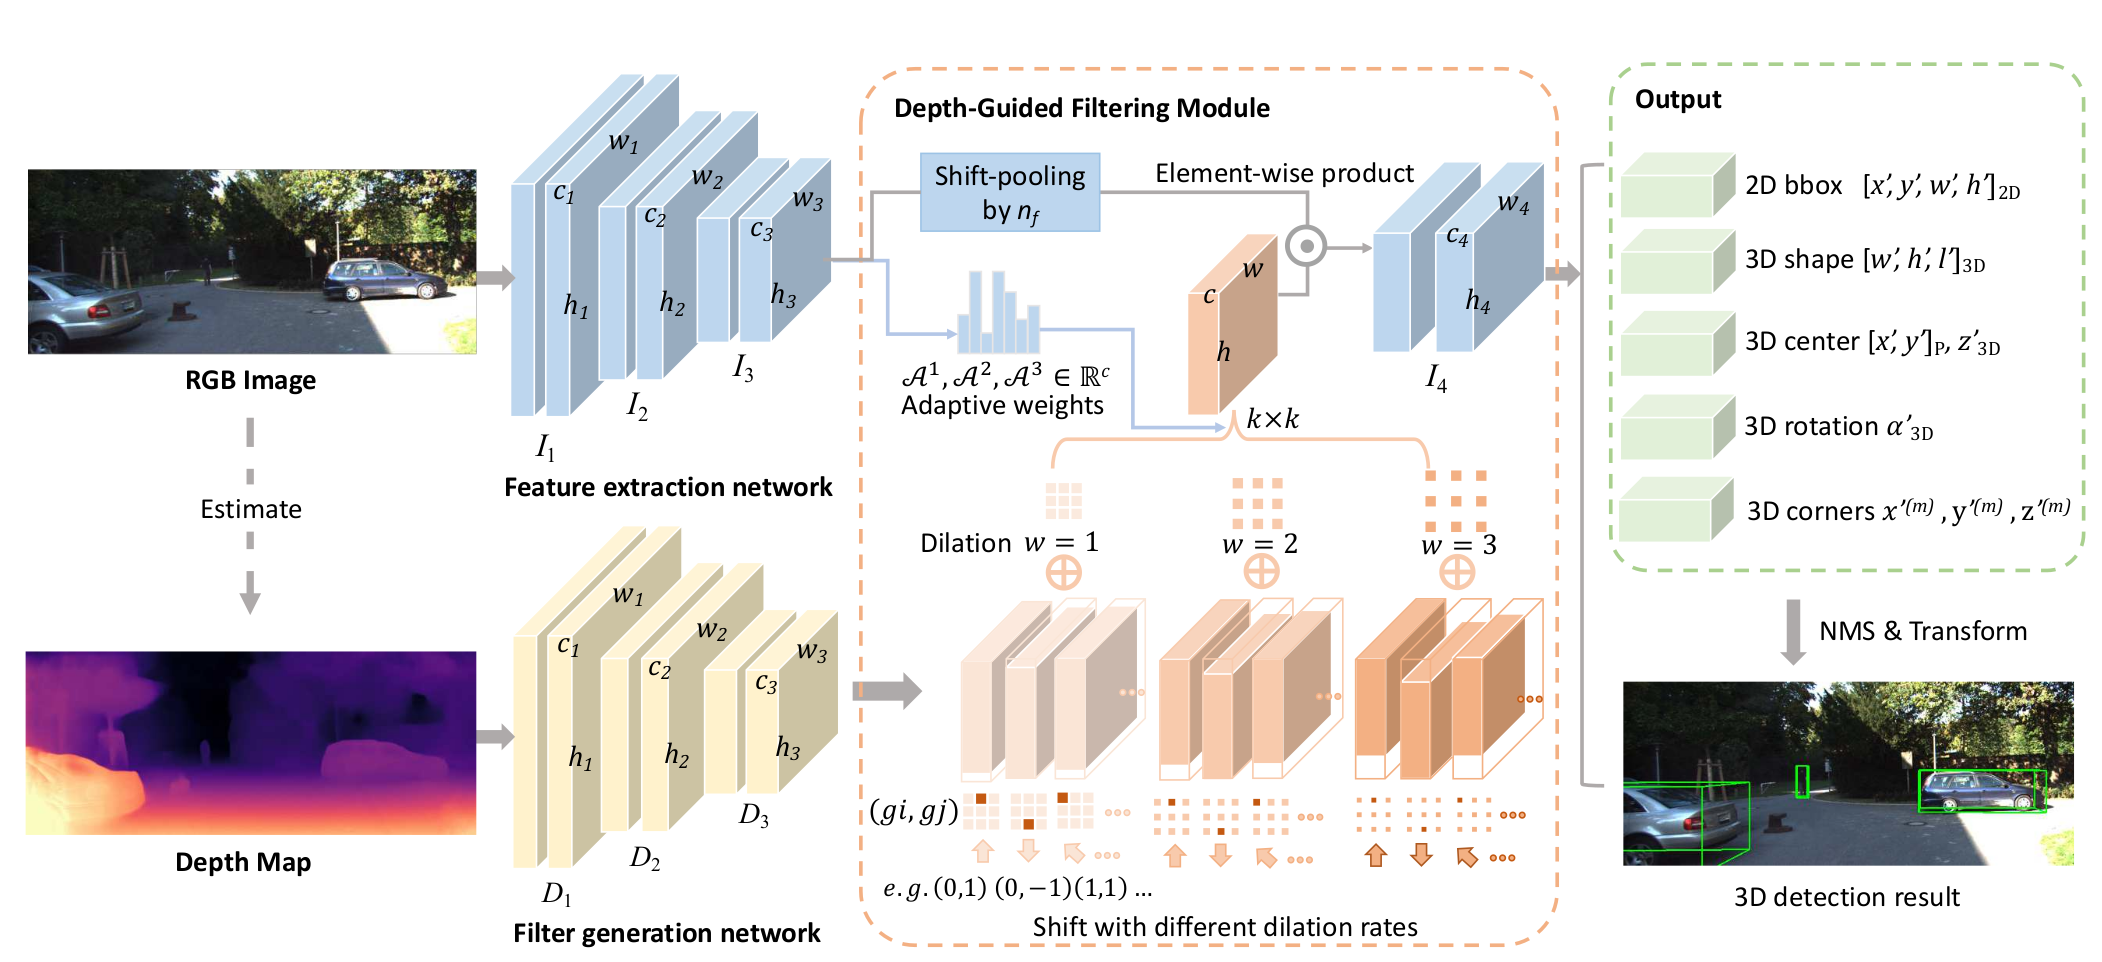
\includegraphics[width=\textwidth]{fig/d4lcn.png}
    \caption*{Fonte: \citeonline{ding2020learning}}
    \label{fig:d4lcn}
\end{figure}

Como métrica de avaliação, seguindo o trabalho de \citeonline{ding2020learning}, serão utilizadas as curvas de precisão-recall com limiar de IoU de 0,7. A base de dados KITTI dispõe as métricas de precisão média interpolada de 11 pontos $AP|_{R_{11}}$.

\section{Considerações Metodológicas}

A metodologia do presente trabalho consiste em três pilares. O primeiro é a comparação entre estimadores de profundidade através de métricas presentes na literatura com o fim de compreender e explorar as capacidades do estado da arte da área e evidenciar suas vantagens e desvantagens em relação a métodos tradicionais. Apesar dos modelos a serem utilizados ainda não terem sido escolhidos, o Apêndice A contém um breve estudo de um modelo estimador baseado em difusão latente, proposto por \citeonline{ke2024repurposing}.

O segundo pilar consiste na aplicação de uma metodologia baseada em processamento digital de imagens para transferir o resultado de estimadores relativos para o espaço métrico, ou seja, com os valores numéricos em unidade de metros. O objetivo é mostrar que com dados auxiliares provenientes de sensores é possível obter distâncias em unidades métricas sem a necessidade de ajuste fino dos modelos, pois esse processo geralmente causa uma adaptação à domínios específicos. 

Por fim, almeja-se comparar os mapas gerados por métodos do estado da arte por meio do desempenho de aplicações práticas, desse modo, mensurando seu comportamento em situações de mundo real. Até o presente momento, a seleção de aplicações seguindo os critérios estabelecidos não foi concluída, havendo somente o estudo de métodos de detecção 3D aplicados a veículos autônomos.